\section{Constraint Check Insertion}
As mentioned before, Redex supports a few different forms of constraint checking; however, for the initial PyRedex implementation only "equality of terms" constraint check will be supported. For example, in pattern `(number\_1 number\_1)` both bound terms must be the same, that is term `(1 1)` matches the pattern but `(1 2)` does not. 

However, the `Match` object does not store multiple bindings for the same symbol and thus assignable symbols seen in the pattern have to be renamed. In the example above, the pattern could become `(number\_1 number\_1\#1)`. Now both bound terms can be stored in the `Match` object.

Now, actual equality checks have to be inserted. Two obvious strategies could be employed here:

\begin{itemize}
\item
Perform constraint checking after the pattern has been matched entirely. For example, `(n\_1 n\_1\#1 n\_2 (Check n\_1 == n\_1\#1))`. The disadvantage of this strategy is that if pattern is large and something goes wrong in the beginning the rest of the pattern is still matched and lots of useless work is done. 

\item
Perform constraint checking the earliest time possible. This implies that by that time both terms have to be matched. Pattern `(n\_1 n\_1\#1 (Check n\_1 == n\_1\#1) n\_2)` is the example of such strategy. The disadvantage of this strategy is that assignable symbols under ellipsis will be checked multiple times. `(((number\_1 ...) (number\_1\#1 ...) (check number\_1 == number\_1\#1)) ...)`
\end{itemize}
The algorithm to be detailed below employs the second strategy.

Finally, since `Match` object now contains extra symbols such as `number\_1\#1` these will have to be removed after successfully matching the pattern.

\subsection{Algorithm}
To be able to insert constraint-checks all symbols to end up in `Match` object have to be known. Since certain symbols will be renamed, need to maintain a mapping between old symbol and new symbol. Additionally, maintain a set to store symbols that will have to be removed. The pattern is traversed recursively. 


\begin{itemize}
\item
\BuiltInPattern and \Nt. Generate a fresh symbol given template string `symbol\_\#`. If generated symbol is `symbol\_\#0` then original symbol is seen for the first time and thus remains unchanged. Otherwise, modify `BuildInPattern` and `Nt` by changing its symbol to a new one. Add new symbol to the set of the symbols to be removed. After processing the pattern, return a mapping `{tag : symbol}` if pattern is `BuildInPattern` or `{nt: symbol}` if pattern is `Nt`.

\item
\LiteralPattern contains to no assignable symbols and thus empty list is returned.

\item
\Repeat. Recursively visit $p$ and return its mapping. 

\item
\PatternSequence. If sequence contains no child patterns, return empty mapping. Otherwise, let `syms` be a mapping returned after visiting the first pattern. For each remaining pattern in the sequence:
	\begin{enumerate}
	\item
	Let `syms2` be a mapping returned after visiting the pattern.
	\item
	Let `syms` be a result of merging `syms` and `syms2` mappings; merging will be discussed below.
	\item
	Let `syms2merge` be a set containing pairs of symbols that have to be checked for equality obtained fter merging `syms` and `syms2` mappings. For each pair of symbols in `syms2merge` add `ConstraintCheck` node to the sequence, exactly after the current pattern. 
	\end{enumerate}

\item
\InHolePattern. Let `syms1`, `syms2` be mappings returned after visiting `pattern1` and `pattern2`, respectively. Let `syms` be a result of merging `syms` and `syms2` mappings, and let `syms2merge` be a set containing pairs of symbols. For each pair of symbols `(s1, s2)` in the set, create `cc\_i` = `ConstraintCheck(s1, s2)` node. Replace InHole pattern with `InHole(pattern1, pattern2, {cc\_0 ... cc\_i ... })`.
\end{itemize}

\subsection{Variable Merging}

Consider pattern `(number\_1 number\_1\#1 number\_1\#2)` and observe that after inserting constraint checks in the following way: `(number\_1 number\_1\#1 (number\_1 == number\_1\#1 ?) number\_1\#2 (number\_1 == number\_1\#2 ?) (number1\#1 == number\_1\#2 ?))` one of the comparisons it the end is superfluous since it's known that `(number\_1 == number\_1\#1)`. Thus, while merging mappings, only one assignable symbol has to be in resulting mapping.

Given two mappings $m1 = {k_i: sym1, k_j: sym2, ...}$ and $m2 = {q_i: sym, q_j: sym}$, compute ${k_0 ... k_i ... k_n}$ intersection ${q_0 ... q_i ... q_n}$. If some $p_i$ is in intersection, retrieve $m1[p_i]$ and $m2[p_i]$ and create pair out of retrieved elements. These symbols will require constraint checking. 

The resulting mapping is constructed in the following way:
\begin{itemize}
\item
If $p_i$ is in intersection, add ${p_i: m2[p_i]}$ to the mapping.
\item
For any $k_i$ that is not in intersection add ${k_i: m1[k_i]}$ to the mapping.
\item
For any $q_i$ that is not in intersection add ${q_i: m2[q_i]}$ to the mapping.
\end{itemize}

\subsection{Example}

\begin{figure}[H]
	\centering
	\makebox[\textwidth][c] { 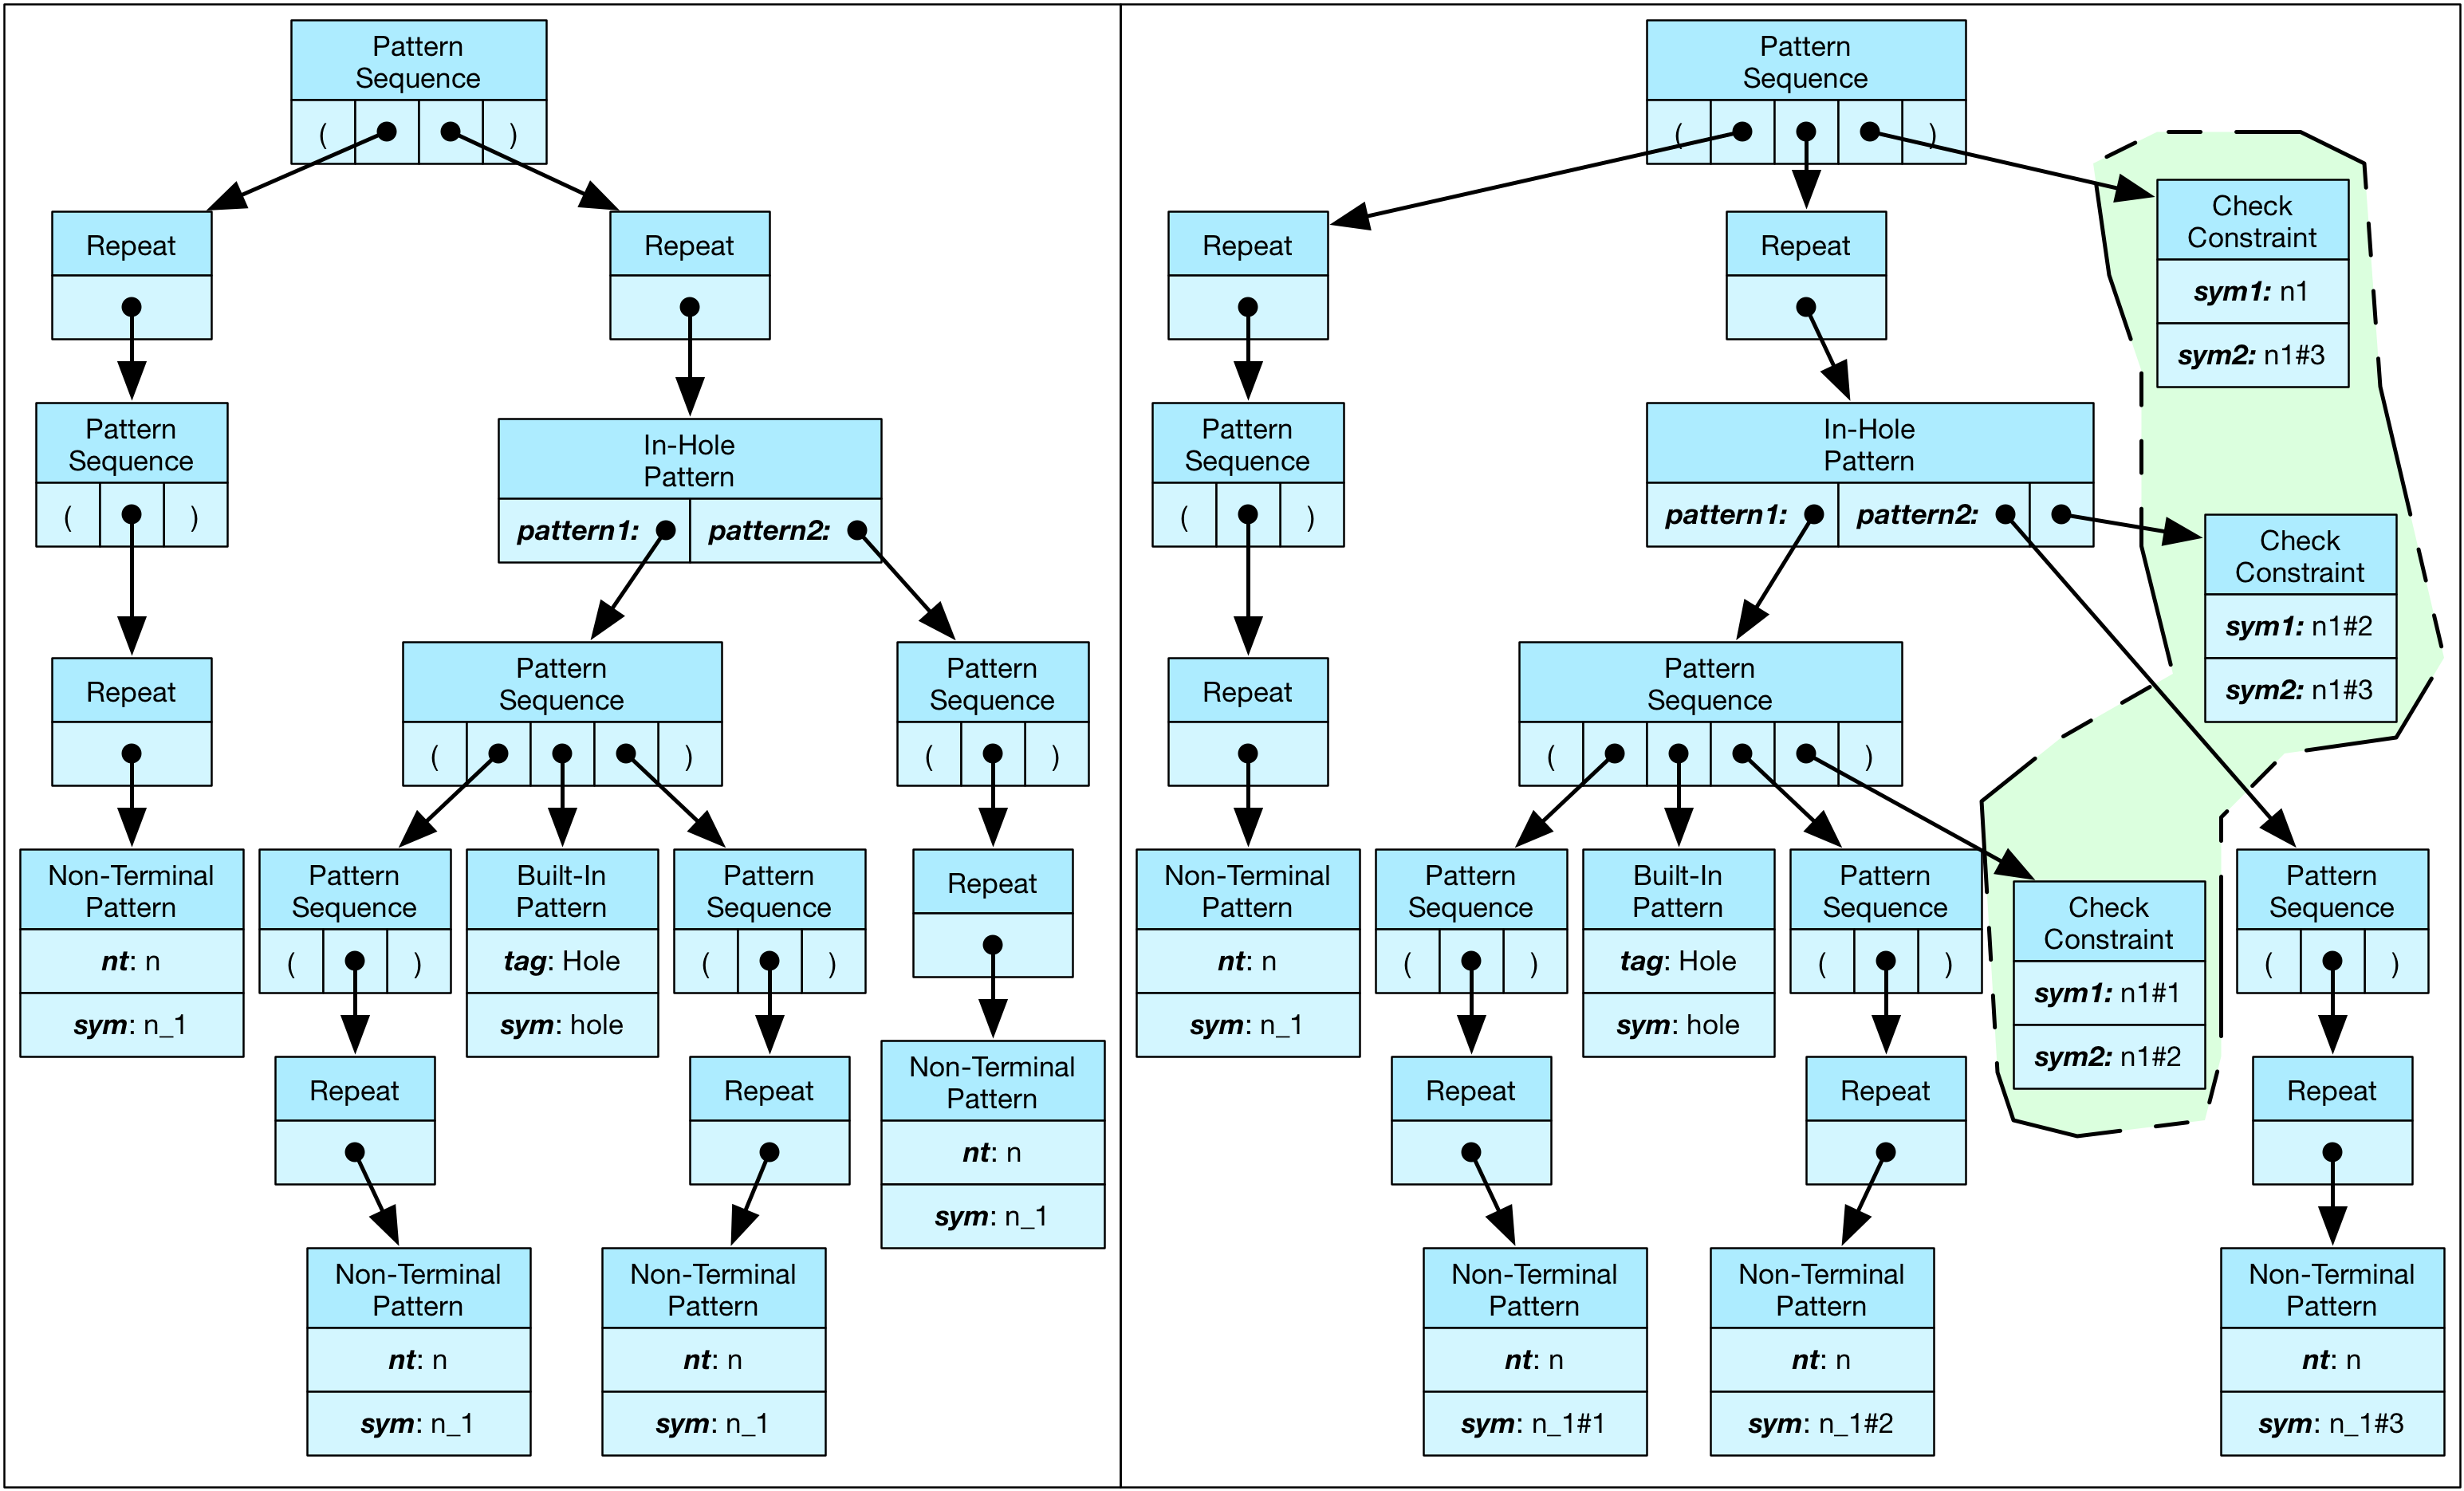
\includegraphics[scale=0.15]{transformation-pattern-constraintcheck.png} }
\caption{Applying transformation to pattern \texttt{((n\_1 ...) ... (in-hole ((n\_1 ...) hole (n\_1 ...)) (n\_1 ...)) ...)}}
\label{transformation-pattern-constraintcheck}
\end{figure}

Figure \ref{transformation-pattern-constraintcheck} shows an effect of described transformation on pattern \texttt{((n\_1 ...) ... (in-hole ((n\_1 ...) hole (n\_1 ...)) (n\_1 ...)) ...)}. Notice that all occurences of \texttt{n\_1} have ellipsis depth of two. The first occurence of \texttt{n\_1} goes unmodified. Then, when processing the first pattern inside \texttt{in-hole} pattern, there are two occurences of \texttt{n\_1}. The first occurence is renamed to \texttt{n\_1\#1}, the second to \texttt{n\_1\#2}, and \texttt{CheckConstraint(n\_1\#1, n\_1\#2)} is appended to the \texttt{PatternSequence}. The final occurence of \texttt{n\_1} is seen in the second pattern of \texttt{in-hole} and is renamed to \texttt{n\_1\#3}. \texttt{CheckConstraint(n\_1\#2, n\_1\#3)} is then added to the \texttt{in-hole}. Finally after exiting \texttt{in-hole}, \texttt{CheckConstraint(n\_1, n\_1\#3)} is appended to \texttt{PatternSequence}.


